%
% 22 Aug 01 - Mike: Some updates for pa-risc changes (e.g. ALIGNMENT etc)
% 22 Oct 01 - Mike: Mention when to use INTEGER.16 etc in RETURNS section of PAL
%

\chapter{Procedure Abstraction Recovery}
\label{ch-call}

{\small
\begin{flushright}
Design and documentation: Cristina [Mar 99], Doug [Aug 1999],
	Mike [Jun 00]; Implementation: Doug [c.99]
\end{flushright} 
}

Functions\footnote{The terms {\it function} and {\it procedure}
are used interchangeabley in this document.} in source code
have a representation in object code that is specific to a given
operating system and hardware architecture combination. For these
object level functions to interoperate with each other, they must
conform to a format described in an Application Binary Interface
(ABI). Compiler writers need to adhere to the ABI if their generated
code is to be compatible with that generated by other compilers. This
constraint is only imposed on functions that are to be available
externally. However, most compilers adhere to the ABI format for
all generated code.

The aim of this work is to use the relevant parts of the ABI to
recover a source code like representation of procedural aspects of
object code. This allows us to abstract from machine dependencies;
for example, in the way that parameters are passed to a procedure,
how values are returned and how local variables are represented.

In particular, we aim to recover the following high level constructs:

\begin{itemize}
\item Signatures for functions (e.g. {\tt integer add(integer, integer)} )
\item High level function invocations: (e.g. {\tt var1 := add(5,var2)} )
\item High level return statements (e.g. {\tt return var1} )
\end{itemize}

The types considered so far are:
\begin{itemize}
\item integer (possibly with a size if found useful)
\item address (pointer to instruction or to data)
\item float (with a size: 1 (single), 2 (double), 4 (quad))
\end{itemize}
This chapter does not deal with the recovery of these low-level types 
(see Chapter~\ref{ch-type}); you need assume that only they exist for now.


\section{Specifications to Support Procedure Abstraction}
\label{sec-callConvSpec}

The Unix System V ABI~\cite{Unix90} describes the application
binary interface rules to be followed on different machines
when implementing Unix System V.  The SPARC~\cite{Unix90b} and
Intel~\cite{Unix90c} processor supplements describe machine-specific
rules to be followed as part of implementing the ABI interface.
Such rules include how to pass parameters to a procedure and how
to return value(s) from a function.  It also describes  the stack
frame and how values on it change during a call.  For SPARC,
machine dependencies such as the register window mechanism are
also explained.

When a compiler generates code for a function call, it first needs
to determine where to pass the parameters (either on registers
or the stack) and place them on the appropriate locations, it
then emits a call to the destination address for the function,
the called function sets up its stack frame and allocates enough
space for local variables and any other space that the ABI may
require it to allocate, then the code for the rest of the function
is emitted.  On function return, a returned value needs to be placed
on certain location(s) and the stack frame needs to be restored to
its original form prior to returning.  Once returned, the caller
determines whether to move the returned value to a register or a
variable as needed.

The above description can be summarized in terms of the caller's
and callee's prologue and epilogue.  The caller's prologue places
the actual arguments and invokes (calls) the function.  The callee's
prologue sets up the stack frame.  The callee's epilogue places the
return value, restores the stack frame and returns.  The caller's
epilogue decides what to do with the returned value.

A calling convention language, CCL~\cite{Bail95}, was developed to
specify calling conventions for different languages and compilers.
The language is used as part of a retargetable compiler and as such
makes use of knowledge known at compile time, such as the number
of arguments passed to a function and the types of such arguments.

At the machine-code level, the types of arguments are unknown until
analysis is performed on them.  Using a specification based on types
does not aid in determining their types.  For example, the FSA in
Figure~\ref{fig-callfsaeg} states that for a particular machine, the
first integer argument is passed on register \texttt{\%o0} and the
second integer argument on register \texttt{\%o1}, or alternatively,
a double floating point argument can be passed in both \texttt{\%o0}
and \texttt{\%o1}.  Although this makes sense from a compiler's point
of view, in machine code we do not see a difference between storing
integers, addresses or double floats in registers \texttt{\%o0}
and \texttt{\%o1}.  The only useful information to us is the fact
that the registers \texttt{\%o0} and \texttt{\%o1} are used to pass
arguments.  Later analysis on the usage of the passed arguments may
determine the difference between integer and double float arguments.

\centerfigbegin
\resizebox{4cm}{!}{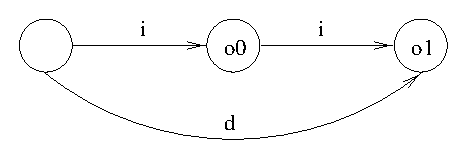
\includegraphics{figures/callfsaeg.eps}}
\centerfigend{fig-callfsaeg}{Sample FSA to Place Integer and Double 
	Floating Point Arguments on Registers}

Given the inadequacy of CCL for out task, we have developed two
new specification languages to support our analysis. The first,
IPL\footnote{\it Keep those acronyms coming!!} (instruction
pattern language) supports the specification of the instruction
sequences from which the caller and callee prologues and epilogues
are composed. IPL is an extension of SLED~\cite{Rams94b}, a language
to support descriptions of machine instruction syntax. IPL extends
SLED to provide support for regular expressions to the language where
the atoms of an expression are individual instructions. The second
language we have developed is PAL (procedure abstraction language).
which provides a means for specifying the calling convention and
other procedure aspects of object code as specified in an ABI.

The following sections demonstrate the use of these
specification languages for the SPARC and Intel platforms. More
detailed descriptions of the languages are given in the \uqbt\ 
source code. 


\section*{SPARC}

The standard stack frame for a single SPARC procedure is composed
of (from low to high addresses) a 16-word area to save the register
window, one word to put the address of a struct/union to return by a
callee, 6 words for a callee to save the first 6 arguments (passed
in registers) to the stack, $n$ words for output arguments 7 and
above, and an area to store locals.  Figure~\ref{fig-stkfrmSparc}
shows the standard stack frame for SPARC.

\centerfigbegin
\resizebox{8cm}{!}{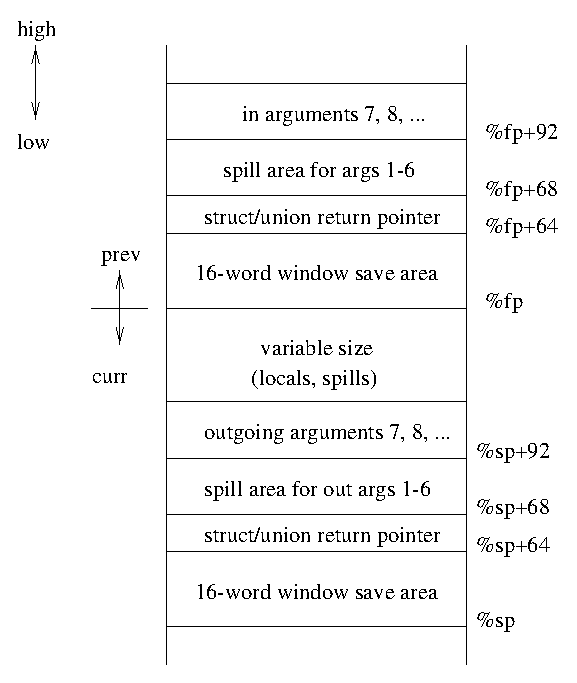
\includegraphics{figures/stkfrm-sparc.eps}}
\centerfigend{fig-stkfrmSparc}{Standard Stack Frame for SPARC Code.
The indexes and register's are given from the context of the callee.}


\subsection{Prologues and Epilogues}

Prior to specifying the prologues and epilogues, it is convenient
to introduce symbolic names for register encodings\footnote{This
is analogous to the {\tt names} construct in SLED.}. For example,
the symbolic name for register 24 on SPARC is {\tt \%o0}. The
set of names defined for SPARC are shown below.

\begin{verbatim}
NAMES
    SP = 14
    FP = 30
    o0 = 8
    i0 = 24
    i7 = 31
    o7 = 15
    g0 = 0
\end{verbatim}

On the SPARC, there are two different ways of invoking a function
based on the return type of the function.  A \texttt{call}
instruction is always used. If the return value is a structure,
union or a quad floating point value, the instruction following the
delayed instruction of the \texttt{call} needs to be a \texttt{unimp}
instruction.  The immediate 22 bits of the \texttt{unimp} are used
to specify the size of the returned value\footnote{Not all compilers
(e.g. gcc) make use of this information to generate runtime size
checking code.}.

\begin{verbatim}
PATTERNS
    CALLER_PROLOGUE std_call addr IS
        call__ (addr)

    CALLER_PROLOGUE struct_call addr IS
        call__ (addr); 
        <4>;  # any 4 byte instruction
        UNIMP (imm22)
\end{verbatim}

The callee prologues that have been identified to date are shown
below. The first two are used when the size of the stack to be
allocated fits into a 13 bit immediate operand. The first one effects
a change to the register window (i.e. allocates a new set of {\it
local} and {\it out} registers) where as the second doesn't. The last
two are analogs of the first two and handle procedures that allocate
a stack whose size cannot be stored in a 13 bit number. A procedure
may not have a prologue at all, as in the case of a leaf procedure
(see page 198 of~\cite{Sparc8}) that doesn't require any stack space.

{\it Note: The last two patterns shown here cannot be used yet as
the pattern parser cannot handle equations or local variables. See
\S\ref{sec:future_work} for a complete description of what is yet
to be implemented to support procedure recovery.}

\begin{verbatim}
    CALLEE_PROLOGUE new_reg_win locals IS
        SAVE ($SP, imode(locals), $SP)

    CALLEE_PROLOGUE same_reg_win locals IS
        ADD ($SP, imode(locals), $SP)

    CALLEE_PROLOGUE new_reg_win_large locals { locals = hiVal+lowVal } IS
        sethi(hiVal,reg);
        ADD (reg, imode(lowVal), reg);
        SAVE ($SP, rmode(reg), $SP)

    CALLEE_PROLOGUE same_reg_win_large locals { locals = hiVal+lowVal } IS
        sethi(hiVal,reg);
        ADD (reg, imode(lowVal), reg);
        SAVE ($SP, rmode(reg), $SP)
\end{verbatim}

The callee epilogue for a procedure on SPARC depends on the following
factors:

\begin{itemize}
\item Does it return an aggregate value?
\item Is it a leaf procedure?
\item Is the value to be returned (if any) already in the right
      location?
\item Has it allocated its own stack?
\end{itemize}

While most combinations of these factors are legal, the majority
of programs will only use a limited subset of the possibile
combinations.  The most common represents a standard return from
a non-leaf procedure (and hence resets the register window). The
value to be returned is already in the expected location ({\tt \%o0}
in this case). The alternatives for the first instruction (i.e. the
actual transfer of control) represent the cases of a scalar (or void)
return value and an aggregate return value respectively.

\begin{verbatim}
    CALLEE_EPILOGUE std_ret IS
        [ ret() |
          JMPL (dispA ($i7, 12), $g0) ];
        restore_()
\end{verbatim}

Two other common combinations are similar to the above except the
value to be returned is moved into the expected location by the
{\tt restore} instruction.

\begin{verbatim}
    CALLEE_EPILOGUE ret_reg_val rs1, rs2 IS
        [ ret() |
          JMPL (dispA ($i7, 12), $g0) ];
        RESTORE (rs1, rmode(rs2), $o0)

    CALLEE_EPILOGUE ret_imm_val rs1, imm IS
        ret();
        RESTORE (rs1, imode(imm), $o0)
\end{verbatim}

Lastly, a leaf procedure usually returns with a {\tt retl}
instruction when returning a void or scalar value or a {\tt jmpl}
instruction when returning an aggregate value. The extra offset from
the calling address in the latter case is to skip the {\tt unimp}
instruction discussed previously.

\begin{verbatim}
    CALLEE_EPILOGUE leaf_ret IS
        [ retl() |
          JMPL (dispA ($o7, 12), $g0) ];
        { SUB ($SP, imode(?), $SP) }
\end{verbatim}

Once the callee returns, any return values are in the right place
and the stack has been restored, so there is no caller epilogue.

The prologues and epilogues presented in this section are the basis
for the PAL specification. The PAL specification encapsulates the
information present in the ABI that describes how parameters are
passed and values returned, where locals are stored and any other
architecture specific information. The following sections present the
sections of the PAL specification for SPARC ABI compliant programs.

\subsection{Frame Abstraction}

To simplify a PAL specification, the first section specifies how to
abstract frame and stack relative address by converting them to be in
terms of a single fixed point, the abstract frame pointer (AFP or
{\tt \%afp}).  Typically, this point should be the value of the stack
pointer after the callee prologue (if any) has been effected as this
is when the abstraction specified takes place. On SPARC, {\tt \%afp}
is indeed initialised to the stack pointer (i.e. {\tt \%sp}). The
substitutions to convert other frame and stack relative addresses to
{\tt \%afp} relative addresses is specified in terms of the callee
prologues previously specified. The only two\footnote{Well four, if
you consider the prologues we can't yet handle.} callee prologues on
SPARC are similar enough that the same substitution for the frame
pointer (i.e. {\tt \%fp}) can be used.  The analysis tracks any
changes to either {\tt \%sp} or {\tt \%fp} throughout the procedure
and updates their respective substitutions correspondingly.

\begin{verbatim}
FRAME ABSTRACTION
    INIT = %sp
    new_reg_win
    same_reg_win
    {
        %fp -> %afp - locals
    }
\end{verbatim}


\subsection{Local Variables}
Local variables are stored within a procedure's stack frame. The size
of this stack frame can be derived from a callee prologue (\textit{We
are assuming that this is always true}). The example below states
that on SPARC, the amount of space (in bytes) allocated for local
variables is equal to the value of the {\tt locals} parameter of
the {\tt new\_reg\_win} and {\tt same\_reg\_win} callee epilogues.

\begin{verbatim}
LOCALS
    new_reg_win
    same_reg_win
    {
        locals
    }
\end{verbatim}

{\it Ideally, we would like to recognise any access addresses within
the portion of the stack frame used for local variables. However,
given the problem of aliasing this is non-trivial and requires
extensive analysis. Even with such analysis, there is no guarantee
that all such references will be detected. The approach we take is
simpler and completely reliable. The user specifies how to derive
the size of the block of memory allocated for locals from the callee
prologue\footnote{I am assuming that this will always be possible}.}

\subsection{Parameter Locations}

As discussed in \S\ref{sec-callConvSpec}, at the machine-code
level we cannot distinguish the variables and types that were used
when placing parameters on appropriate parameter-passing locations.
On SPARC, all parameters are copied by instances of one word, hence,
a double floating point value is copied as two words, in exactly
the same way as two individual integers or even two addresses are
copied.  Low-level type information can be retrieved from usage at
the called site.

The ABI specifies which locations are used for passing parameters,
and the order of usage of those locations. The means by which
the parameters are referenced across a call boundary is dependent
upon the {\it view change} effected by a call. The view change can
be thought of as the low level analog of using actual and formal
parameters in source code. That is, the same parameter is referenced
differently depending on whether the context of the reference is
the call instruction or in the called procedure.

To account for the view change effected by a call, we specify
parameter locations from the both context of the caller (outgoing
parameters) and the callee (incoming parameters).

The first part of the parameters section specifies where the outgoing
parameters are found. This is acheived by attaching a parameters
specification to the {\tt CALLER} keyword.

\begin{verbatim}
PARAMETERS
    CALLER
    {
        AGGREGATE -> m[%afp + 64]
        REGISTERS -> %o0 %o1 %o2 %o3 %o4 %o5
        STACK     -> BASE = [%afp + 92]
                     OFFSET = 4
    }
\end{verbatim}

Each sub-clause is optional but if present, it must obey the
ordering implied in the above example (i.e. {\tt AGGREGATE} before
{\tt REGISTERS} before {\tt STACK}). This ordering complies with
how parameters are passed on all architectures we have encountered.

The \texttt{AGGREGATE} sub-clause states where the address of an
aggregate value to be returned is found. This location will only
be used by calls to procedures that actually return a struct.
Additionally, only some architectures (such as SPARC) make use of
a special location for this purpose. Others (e.g. Intel) simply
pass it as the first parameter\footnote{This effectively makes it a
``hidden" argument in that it doesn't correspond to any source code
level parameter.}.

The {\tt REGISTERS} sub-clause states that registers {\tt \%o0..\%o5}
(in that order) are used for the first 6 parameters (after the
aggregate address parameter if used). Any extra parameters are
passed via the stack and are found in locations {\tt m[\%afp + 92],
m[\%afp + 96], m[\%afp + 100], ...} as specified by the {\tt STACK}
subclause.

In addition, there can be an {\tt ALIGNMENT} sub-clause, after the
{\tt STACK} and before the closing curly bracket. {\tt REGISTERS}
can also have a
type before it, to designate the type of parameters that the given
registers can hold. The type can be one of {\tt INTEGER}, {\tt FLOAT},
or {\tt DOUBLE}. Where a type is not given, as above, {\tt INTEGER} is
assumed. Where more than one type of register is given, they must be
in the order {\tt INTEGER}, {\tt FLOAT}, then {\tt DOUBLE} (with any or
all being optional). For example, for HP pa-risc:

\begin{verbatim}
PARAMETERS
    CALLER
    {
        AGGREGATE -> m[%r28]
        INTEGER REGISTERS -> %r26 %r25 %r24 %r23
        FLOAT   REGISTERS -> %fr4 %fr5 %fr6 %fr7
        DOUBLE  REGISTERS -> %fd5 %fd7
        STACK -> BASE = [%afp - 52]
                 OFFSET = -4
        DOUBLE ALIGNMENT 8 BYTES
    }

\end{verbatim}

When multiple {\tt REGISTERS} are given as above, they are considered to
operate ``in parallel". In other words, when the first parameter goes into
either \%r26 or \%fr4, this ``parameter slot" is ``used up", and so the next
parameter goes into register \%r25, \%fr5, or \%fd7, depending on the type.
If the first parameter is a {\tt DOUBLE}, then two parameter slots are
used up.

The {\tt ALIGNMENT} sub-clause states that parameters of type {\tt DOUBLE}
(64 bit floating point) are aligned on 8 byte boundaries. This applies to
registers and stack locations alike; that's why there are only two
{\tt DOUBLE REGISTERS}. As an example, if a pa-risc function took an
integer, a double, and an integer, then even though these could easily
fit into three registers, they are actually placed in registers \%r26,
\%fd7, and stack location [\%afp-52]. The alignment of the double parameter
``skips" register \%r25, and because doubles are twice as big as integers,
using \%fd7 ``uses up" the parameter slots for \%r24 and \%r23. So the third
parameter has to go to the stack. If there was a fourth parameter of type
{\tt DOUBLE}, it would go to [\%afp-64] (and the other half at [\%afp-60]),
skipping the word at [\%afp-56] to keep the argument aligned on 8 byte
boundaries.

This indicates a significant difference between SPARC and pa-risc architectures.
On the non aligned SPARC, a {\tt DOUBLE} parameter could be split between
an integer register and the stack. On the aligned pa-risc, such splits
can't happen. On the other hand, ``gaps'' in the parameters can be seen
in pa-risc programs, while these will never be seen on the SPARC.

Outgoing parameters are always placed at the same locations. Incoming
parameters however, depend upon the prologue of the procedure being
invoked as it is this prologue that effects the aforementioned
view change. Stack parameters may be found at different offsets
after allocation of the procedure's stack frame. Also, a register
window change will mean that some registers will now accessed via
different register names.

On SPARC, the {\tt new\_reg\_win} prologue changes the register
window, effectively renaming the eight output registers ({\tt
\%o0..\%o7}) to the eight input registers ({\tt \%i0..\%i7}).

\begin{verbatim}
    new_reg_win
    {
        AGGREGATE -> m[%afp - locals + 64]
        REGISTERS -> %i0 %i1 %i2 %i3 %i4 %i5
        STACK     -> BASE = [%afp - locals + 92] 
                     OFFSET = 4
    }
\end{verbatim}

The other prologue, {\tt same\_reg\_win}, doesn't change the register
window but changes the stack offsets.

\begin{verbatim}
	same_reg_win
    {
        AGGREGATE -> m[%afp - locals + 64]
        REGISTERS -> %o0 %o1 %o2 %o3 %o4 %o5
        STACK     -> BASE = [%afp - locals + 92] 
                     OFFSET = 4
    }
\end{verbatim}

\subsection{Return Locations}

Return values need to be placed in specific registers depending on
the type of the value to be returned. As with incoming parameters,
the locations used will depend on the view change effected by the
prologue of the procedure doing the return.

\begin{verbatim}
RETURNS
    ret_reg_val
    ret_imm_val
    leaf_ret
    CALLER
    {
        INTEGER   IN %o0
        ADDRESS   IN %o0
        FLOAT     IN %f0
        DOUBLE    IN %f0to1
    }
    std_ret
    {
        INTEGER   IN %i0
        ADDRESS   IN %i0
        FLOAT     IN %f0
        DOUBLE    IN %f0to1
    }
\end{verbatim}

Note that double refers to a 64 bit float and as such is returned in
a synthetic register that denotes two 32 bit registers.

Once again, the {\tt CALLER} keyword indicates that the accompanying
specification is from a caller's perspective. In this case it is
where a caller will receive a returned value.

\subsection{Accesses to a Parent's Stack}

This is the first (and so far, only) section that is optional in
that not all architectures will require it.

On SPARC, a procedure may write to a certain portion of its parent's
stack frame. This capability is provided primarily so that parameters
in registers can be spilled to the stack resulting in all parameters
being located in a contiguous segment of memory. This is typically
required when the source code uses variable argument lists or
takes the address of a parameter. Compiler writers can leverage
this capability and use this portion of the parent's stack as
space for temporary variables. In order to abstract away from
referring stack locations, we replace accesses to these addresses
with variables. To do so requires that these addresses are specified
in a PAL specification as shown below.

\begin{verbatim}
PARENT STACK
    new_reg_win
    same_reg_win
    {
        %afp - locals + 68 TO %afp - locals + 88 STEP 4
    }
\end{verbatim}

\section*{Intel}

The standard stack frame of a procedure includes space for arguments,
the return address of the caller, the frame pointer value of the
caller (\texttt{\%ebp}), and enough space for local variables and
spilled values (including registers that need to be preserved across
procedure calls).  Figure~\ref{fig-stkfrmIntel} shows the standard
stack frame for Intel code.

\centerfigbegin
\resizebox{10cm}{!}{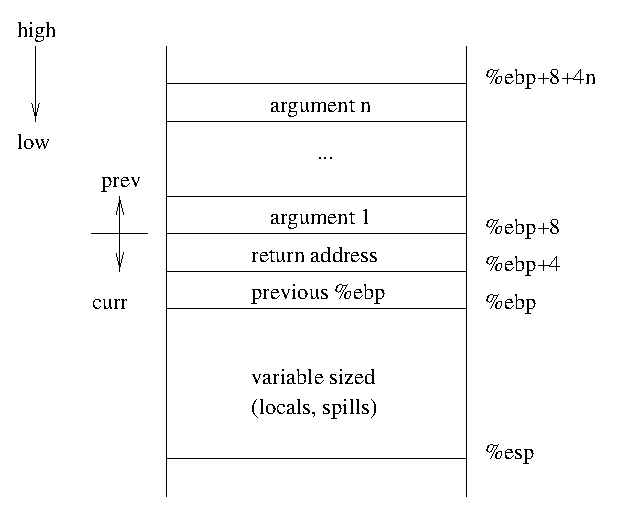
\includegraphics{figures/stkfrm-intel.eps}}
\centerfigend{fig-stkfrmIntel}{Standard Stack Frame for Intel Code}

\subsection{Prologues and Epilogues}

As with SPARC, we start the prologue and epilogue specification by
declaring symbolic names for the register encodings.

\begin{verbatim}
NAMES
    EAX = 0
    ECX = 1
    EDX = 2
    EBX = 3
    ESP = 4
    EBP = 5
    ESI = 6
    EDI = 7
\end{verbatim}

On Intel x86, there is only one way to invoke a procedure, even if
the procedure is to return a value or a structure.  The \texttt{call}
instruction is used, and although this assembly instruction maps to
one of five different machine instructions, only one is used for
direct calls; the intra-segment direct call {\tt CALL\_.JVOD}.  For
indirect calls (i.e. via a register), the intra-segment indirect call
is used (CALL.EVOD modrm).  Indirect calls require extra analysis to
determine the target address of the call; this is addressed in a
different document.  For now assume all calls are direct.

\begin{verbatim}
PATTERNS
    CALLER_PROLOGUE std_call addr IS
        CALL.Jvod (addr)
\end{verbatim}

The most common callee prologue sets up the frame base pointer and
the stack pointer, as well as optionally allocating space on the
stack for locals and spilled values.  Further, the contents of
registers \texttt{\%edi}, \texttt{\%esi} and \texttt{\%ebx} need to
be preserved across procedure calls.  That is, if these registers are
used by the callee, they need to be spilled to the stack as part of
the prologue. 

\begin{verbatim}
    CALLEE_PROLOGUE std_entry locals=0, regs IS
        PUSHod ($EBP);
        MOVrmod ($EBP, Reg($ESP));
        { SUBiodb (Reg ($ESP), locals) |
          SUBid    (Reg ($ESP), locals) };
        { [ PUSHod ($ESI) |
            PUSHod ($EBX) |
            PUSHod ($EDI) ] *regs <1..3> }
\end{verbatim}

In the case where an aggregate value is to be returned, the address
at which this value is to be stored can be passed as the first
(hidden) argument of the call. It has been noted that some compilers
move this address into {\tt \%eax} as part of the prologue\footnote{
Initially this was believed to be an optimisation as the address of a
returned aggregate value must be in {\tt \%eax} upon returning from
the procedure.  However, analysis shows that this is not the case as
these procedures subsequently write to {\tt \%eax} before doing a
return. It does mean the simple form of {\tt RET} can be used in the
epilogue but I'm not sure that this can be classified as an
optimisation}.

\begin{verbatim}
    CALLEE_PROLOGUE struct_ptr locals, regs IS
        POPod ($EAX);
        XCHG.Ev.Gvod (E (Base ($ESP)), $EAX);
        @std_entry (locals, regs)  
\end{verbatim}

The standard epilogue restores any of the registers that need to be
preserved across a procedure call (i.e. \texttt{\%ebx},
\texttt{\%esi} or \texttt{\%edi}), restores the stack pointer and the
frame pointer, and returns to the caller's return address.  Restoring
registers to be preserved across procedure calls can be done in one
of two ways; by popping them from the stack, or by indexing into the
stack directly.  It has also been noticed that some compilers
generate a \texttt{LEAod} (load effective address) at the start of
the epilogue, to ensure the stack pointer is pointing to the right
address, even if this instruction is redundant (as has been seen in
gcc -O2 generated code). The {\tt RET.Iw} instruction is used to
remove the address of a returned aggregate value if this hasn't
already been done so by the prologue.

\begin{verbatim}
    CALLEE_EPILOGUE std_ret IS
        { LEAod ($ESP, Disp8(?,$EBP)) };
        { [ MOVrmod ($EBX, E( Disp8(?,$EBP))) |
            MOVrmod ($ESI, E( Disp8(?,$EBP))) |
            MOVrmod ($EDI, E( Disp8(?,$EBP))) ] * <1..3>
          |
          [ POPod ($EBX) |
            POPod ($ESI) |
            POPod ($EDI) ] *<1..3> };
        [ LEAVE () | [ MOVrmod ($ESP, Reg($EBP)); POPod ($EBP) ]];
        [ RET () | RET.Iw (?) ]
\end{verbatim}

Simple procedures that use no stack and take no parameters have a
very basic epilogue.

\begin{verbatim}
    CALLEE_EPILOGUE simple_ret IS
        RET () | RET.Iw (?)
\end{verbatim}
 

Upon return from a call, the stack needs to be restored by the caller in 
order to remove the parameters that were passed on the stack.  
Restoring of the stack is done by modifying the value of the stack
pointer by a certain number of bytes, or by popping values from the
stack a certain number of times (4 bytes at a time).  Either way 
will tell us how many bytes are restored from the stack. 

\begin{verbatim}
    CALLER_EPILOGUE clear_stack n IS
        [ ADDiodb (Reg($ESP),n) | ADDid (Reg($ESP),n) ] |
        [ POPod ($EAX) |
          POPod ($EBX) |
          POPod ($ECX) |
          POPod ($EDX) |
          POPod ($ESI) |
          POPod ($EDI) |
          POPod ($EBP) ] * n <1..7>
\end{verbatim}

\subsection{Frame Abstraction}

On Intel, we initialise {\tt \%afp} to be the value of {\tt \%esp}
after the prologue (if any) has been executed. As with SPARC, a
similiar substitution is specified for the frame pointer.

\begin{verbatim}
FRAME ABSTRACTION
    INIT = %esp
    std_entry
    struct_ptr
    {
        %ebp -> %afp + (regs * 4) + locals
    }
\end{verbatim}


\subsection{Local Variables}
The size of the block of memory allocated for local variables will
be the initial increment to the stack pointer plus the number of
bytes pushed to the stack when preserving registers.

\begin{verbatim}
LOCALS
    std_entry
    struct_ptr
   {
      locals + (regs * 4)
   }
\end{verbatim}

\subsection{Parameter Locations}

Outgoing parameters on Intel are always found at the bottom of the
stack. Given that we can't statically specify where the bottom of
the stack is, we simply choose a fixed stack address. Accompanied
with a negative offset, this implies that all address that are at
multiples of this offset from are potential parameter locations. The
analysis will then determine which of these locations are live at a
call and recovery as many as it needs to match the signature of the
callee, starting at the lowest addresses. This is exactly the same
approach taken with stack parameters on SPARC but the fixed point
specified in the SPARC PAL specification just happens to be the lowest
address (as implied by the positive offset accompanying it).

\begin{verbatim}
PARAMETERS
    CALLER
    {
        STACK     -> BASE = [%afp - 4]
                     OFFSET = -4
    }
\end{verbatim}

Procedures with the {\tt std\_entry} prologue will find their incoming
parameters at positive offset from the frame pointer. Of course, the
specification is given in terms of {\tt \%afp} as we want to abstract
away from concepts such as a frame pointer.

\begin{verbatim}
    std_entry
    {
        STACK     -> BASE = [%afp + locals + (regs * 4) + 8]
                     OFFSET = 4
    }
\end{verbatim}

The {\tt struct\_ptr} prologue contains the side effect of popping
the address of the aggregate value to be returned from the stack into
{\tt \%eax}\footnote{It it turns out that some other register is used,
then the register used can be parameterised in the pattern and the
parameter name used here instead of {\tt \%eax}.}. As such, the
incoming parameters specification for procedures prefixed with this
prologue require an {\tt AGGREGATE} location to be included.

\begin{verbatim}
    struct_ptr
    {
        AGGREGATE -> %eax
        STACK     -> BASE = [%afp + locals + (regs * 4) + 8]
                     OFFSET = 4
    }
\end{verbatim}

\subsection{Return Locations}

The RETURNS section specifies where returned values can be found. Again,
there are subsections for each callee prologue, and one for callers, using
the special keyword CALLER. Often the different integer values (byte,
short, int) are returned in the same register. If, and only if, the register
numbers are different for the integral subtypes, then an entry should exist
for INTEGER.16 and so on. On a RISC machine like SPARC, parts of registers
are typically not given different register numbers, so these don't appear:

\begin{verbatim}
RETURNS
# Note: even though functions with save/restore return integer locations in %i0,
# we use the STD_RET_ pseudo instruction for these, which copies %i0 to %o0.
# This simulates the semantics of the restore (for the purposes of return
# location), so we don't need a separate set of locations for these functions
    ret_reg_val
    ret_imm_val
    leaf_ret
    std_ret
    CALLER
    {
        INTEGER.32  IN %o0
        ADDRESS     IN %o0
        FLOAT.32    IN %f0
        FLOAT.64    IN %f0to1
    }
\end{verbatim}

On Intel, all fixed point scalar values are returned in {\tt \%eax},
but the word and byte part of eax is called a different register name.
All floating point values are returned on the top of the floating
point stack. The register number of the top of stack depends on whether
a caller or callee is involved:

\begin{verbatim}
RETURNS
    std_ret
    frameless_epi
    {
        INTEGER.32  IN %eax
        INTEGER.16  IN %ax      # So that functions returning shorts
        INTEGER.8   IN %al      # or chars can be analysed as such
        ADDRESS     IN %eax
        FLOAT.80    IN %st7
    }

    CALLER
    {
        INTEGER.32  IN %eax
        INTEGER.16  IN %ax      # So that functions returning shorts
        INTEGER.8   IN %al      # or chars can be analysed as such
        ADDRESS     IN %eax
        FLOAT.80    IN %st
    }
\end{verbatim}

\subsection{Accesses to a Parent's Stack}

Intel procedures never access any stack locations outside of their
own stack apart from those storing incoming parameters.

\section{Procedure Abstraction Analysis}

The goal of this analysis is to use the specification described in the
preceeding sections to remove any references to stack locations in
object code. Such references will be recovered into either parameters
or local variables. There are 5 steps involved in this analysis:

\begin{enumerate}
\item Replace all stack and frame pointer relative addresses with
  their equivalent {\tt \%afp} relative addresses.
\item Recover the signature (parameters only) of user code procedures.
\item Analyse each call to recover the actual parameters of the call.
  this step also includes recovering the return type of the procedure
  called if it isn't a library procedure.
\item Replace any accesses from within a procedure to locations in its
  parent's stack with accesses to local variables.
\end{enumerate}

This analysis is to be performed only on user procedures; library
procedures will be assumed to have been processed by now, either
through generation of call signatures from header files or through
application of the following analysis to library code.

The following subsection consider each of the above steps in
detail. Throughout this section we will make use of the SPARC
example in Figure~\ref{fig-c_gcd}.  Issues specific to Intel are
discussed in $\S$\ref{sec-callsigIntel}.

\centerfigbegin
{\small
\begin{verbatim}
gcd:                           main:
    save %sp,-112,%sp               save %sp,-112,%sp
    mov %i0,%l0                     mov 10,%o0
    cmp %l0,%i1                     mov 5,%o1
    bge .LL12                       sethi %hi(.LLC0),%l0
    mov %i1,%i0                     call gcd  
    b .LL12                         or %l0,%lo(.LLC0),%l0
    mov %l0,%i0                     mov %o0,%o3
.LL6:                               mov %l0,%o0
    call .rem                       mov 10,%o1
    mov %i0,%o1                     call printf  
    cmp %o0,0                       mov 5,%o2
    bne,a .LL12                     ret
    add %i0,-1,%i0                  restore
    mov %i1,%o0
    call .rem  
    mov %i0,%o1
    cmp %o0,0
    be .LL10
    nop
    add %i0,-1,%i0
.LL12:
    cmp %i0,1
    bg .LL6
    mov %l0,%o0
.LL10:
    ret
    restore
.LLC0:
    "gcd of %d, %d is %d\n"
\end{verbatim}
}
\centerfigend{fig-c_gcd}{SPARC Assembly Code for GCD Program}


\subsection{Recovery of Parameters}
Actual parameters are placed by the caller in one or more of the
locations specified by \texttt{caller parameters}.  The callee
will effect the \texttt{view change} applicable to its prologue, 
and will then use the passed parameters directly or place them 
on the parameter spill area.  Either way, the parameters are 
used before definition within the callee, and this is what 
tells us that the information in that location was setup elsewhere
in the program. 

In the example of Figure~\ref{fig-c_gcd}, \texttt{main} calls 
\texttt{gcd}, using the most frequently used calling convention;  
\texttt{interface1}.  
At the \texttt{call} site, the parameter locations that are live are: 
\begin{verbatim}
     live = {%o0, %o1}
\end{verbatim}
At the callee site, we apply the \texttt{view change} of 
\texttt{callee\_prologue1} to the live parameter locations, the 
stack pointer, and the return address, leading to
\begin{verbatim}
     %o0 -> %i0
     %o1 -> %i1
     %sp -> %fp
     %o7 -> %i7
     %sp -> %sp-112
\end{verbatim}
For \texttt{gcd} we summarize the live-in information for the whole 
procedure based on the parameter locations (view changed).  This gives us
\begin{verbatim}
     liveIn(gcd) = {%i0, %i1}
\end{verbatim}
This information tells us that there are 2 parameters, which match the
two live parameter locations at the call site, hence the actual 
parameters to the call are \texttt{\%o0} and \texttt{\%o1}.  The 
transformed CALL instruction looks like this:
\begin{verbatim}
     CALL gcd [<ret type>] <(%o0,<type>), (%o1,<type>)>
\end{verbatim}

Note that for parameter locations that are on the stack, the 
view change of these looks as follows:
\begin{verbatim}
     %sp+92+n -> %fp+92+n
\end{verbatim}
Hence, accesses to \texttt{\%fp+92+n} at the callee site are 
accesses to parameter locations.  It is also feasible for the
callee site to access these locations using the stack pointer; 
this is needed for leaf routines but it can also be used in 
non-leaf routines: 
\begin{verbatim}
     %sp+(92+simm13)+n
\end{verbatim}
We need to support both views of stack parameter locations.


\subsubsection*{Fixed vs Variable Number of Arguments}
Most procedures take a fixed number of arguments.  However, languages
like C allow for variable number of arguments to be passed at any
one time.  The ABI~\cite{Unix90} does not place any rules on variable 
number of parameters, but states that the calling convention rules need to 
be satisfied; that is, the first 6 word parameters go into registers
and the next go onto the stack.  Disassembled C code shows that 
the first thing the callee does is to move all the register parameters
to the parameter spill area, and then use them all on the stack 
(as the stack parameters are contiguous to the spilled register 
parameters). 

It is not clear that in all cases usage analysis of parameter 
locations at the callee will determine the number of parameters
taken by the callee (think of \texttt{printf}, it can take any
number and the code is bound to be a loop on a string).  
Also, different invocations of the procedure will take different
number of arguments.
\emph{I propose we pass all the live parameter locations at the call
site in the mean time; we will see from the implementation whether
this will cause problems with stack parameter locations.}


\subsection{Recovery of Return Value}
The callee will place a return value on a valid \texttt{callee return}
location.  We note that if anything is placed on a return location,
this location will be live-out of the callee.  
The caller will need to apply the inverse of the \texttt{view change}
to live-out callee locations.  
If the caller is to make any use of a returned value, the location
where it was stored will be used before being re-defined.  Usage is 
commonly in the form of storing to a local variable or using it
as a parameter to another procedure.  
Once this is determined, the callee's RET instruction is set to 
return the relevant return location.
 
For the example of Figure~\ref{fig-c_gcd}, the callee, \texttt{gcd}, 
has only one return location live-out, which matches its \texttt{callee
return} for \texttt{interface1}: 
\begin{verbatim}
     live-out = {%i0}
\end{verbatim}
The caller uses \texttt{\%o0} before definition, hence this is our
return location. 
The callee's RET instruction can now be transformed to: 
\begin{verbatim}
    RET %i0
\end{verbatim}
The caller's CALL instruction can now be transformed into an ASSIGN 
(assignment) instruction as follows: 
\begin{verbatim}
    %o0 = CALL gcd <(%o0,<type>), (%o1,<type>)>
\end{verbatim}

\emph{Should we introduce a HL ASSIGN or shall we use RTL assign 
instead?}

Note that as of 8th September 2000, the return value analysis is done before
the actual parameter analysis. This is because the return value analysis
may cause re-analysis of some of the children, which may impact on the
parameters of the call being considered.

\subsubsection*{Returned Values not Used}
Returned function values are not always used by the caller.  In such
cases, different invocations of the same procedure will show different
return location usage.  In these cases, we go for the more general 
one (i.e. the procedure returns a value) and we annotate each actual 
call with whether the return value is used or not.  In this way, the
signature for the procedure is correct. 


\subsection{Issues Relating to Intel Call Signature Analysis}
\label{sec-callsigIntel}
The nature of Intel passing parameters on the stack means that
optimizing compilers may delay the restoring of the stack until 
after several calls to (different) procedures have been emitted. 
This means that the caller epilogue is optional, and where 
available, it may not necessarily match the number of bytes 
passed as parameters to the caller but may also include bytes
used in a previous call.  We can still make use of liveness 
analysis to determine which arguments are passed to each procedure 
nevertheless.
For the purposes of illustration, we will make use of 
Figure~\ref{fig-gcdIntel}, an optimized version of the GCD program for Intel.

\centerfigbegin
{\small
\begin{verbatim}
gcd:                        main:
    pushl %ebp                  pushl %ebp
    movl %esp,%ebp              movl %esp,%ebp
    pushl %edi                  pushl %esi
    pushl %esi                  pushl %ebx
    pushl %ebx                  movl $10,%esi
    movl 8(%ebp),%ebx           movl $5,%ebx
    movl 12(%ebp),%edi          pushl %ebx
    movl %edi,%esi              pushl %esi
    cmpl %edi,%ebx              call gcd
    jge .L12                    pushl %eax
    movl %ebx,%edi              pushl %ebx
    jmp .L12                    pushl %esi
.L6:                            pushl $.LC0
    movl %ebx,%eax              call printf
    cltd                        leal -8(%ebp),%esp
    idivl %edi                  popl %ebx
    testl %edx,%edx             popl %esi
    jne .L7                     leave
    movl %esi,%eax              ret
    cltd
    idivl %edi
    testl %edx,%edx
    je .L13
.L7:
    decl %edi
.L12:
    cmpl $1,%edi
    jg .L6
.L13:
    movl %edi,%eax
    leal -12(%ebp),%esp
    popl %ebx
    popl %esi
    popl %edi
    leave
    ret  
.LC0:
    "gcd of %d, %d is %d\n"
\end{verbatim}
}
\centerfigend{fig-gcdIntel}{Intel Optimized Assembly Code for GCD Program}

Procedure \texttt{main} calls \texttt{gcd} using the calling convention 
specified in \texttt{interface2} with an immediate value of 12 bytes. 
The calling convention does not include a caller epilogue. 
At the \texttt{call} site, the \emph{parameter locations} that are live are: 
\begin{verbatim}
     live = {[%esp], [%esp+4]}
\end{verbatim}
Applying the \texttt{view change} for \texttt{interface2} to the live
parameter locations we get: 
\begin{verbatim}
     ['%esp]   -> [%esp+20]
     ['%esp+4] -> [%esp+24]
and
     ['%esp]   -> [%ebp+8]
     ['%esp+4] -> [%ebp+12]
\end{verbatim}
Procedure \texttt{gcd} has the following set of parameter locations
live on entry, and return locations live on exit: 
\begin{verbatim}
     liveIn = {[%ebp+8], [%ebp+12]}
     liveOut = {%eax}
\end{verbatim}
The liveIn parameters match the ones that were live on entry, hence 
we can safely assume that 2 words (8 bytes) were passed as arguments.
The call is transformed to the following HL instruction: 
\begin{verbatim}
    CALL gcd [<ret type>] <([%esp],<type>), ([%esp+4],<type>)>
\end{verbatim}
which is further transformed into what was actually placed at those 
stack locations (i.e. this information needs to be stored previously): 
\begin{verbatim}
    CALL gcd [<ret type>] <(%esi,<type>), (%ebx,<type>)>
\end{verbatim}
The liveOut information tells us that \texttt{\%eax} is returned. 
Further, at the caller's site, the value of \texttt{\%eax} is 
used prior to definition.  Even if this value was not used, the ABI 
states that return locations should only be set to a value if they
are intended to return a value, as there is no type checking on 
this interface.  The return instruction in \texttt{gcd} is changed to
\begin{verbatim}
     RET %eax
\end{verbatim}
and the caller's site call is changed to 
\begin{verbatim}
     %eax = CALL gcd <(%esi,<type>), (%ebx,<type>)>
\end{verbatim} 
Although there is no caller epilogue to restore the stack, we have
determined the right arguments to this call.

The next call that \texttt{main} performs is to the library procedure 
\texttt{printf}.  In this case, if we had signatures for \texttt{printf} 
we could only be assured of one fixed parameter (an address) and maybe
some more parameters, as this is a variable argument procedure.  
Also, the calling convention does not specify a caller epilogue in 
this case either, hence we cannot determine exactly how many bytes
are passed on the stack to this call.  The best that can be done is
to pass \emph{all} parameter locations that are live at the call site: 
\begin{verbatim}
     live = {[%esp], [%esp+4], [%esp+8], [%esp+12], [%esp+16], [%esp+20]}
\end{verbatim} 
When replacing this information into the HL call, we get: 
\begin{verbatim}
     CALL printf <(.LC0,<addr>), (%esi,<type>), (%ebx,<type>), (%eax,<type>),
                  (%esi,<type>), (%ebx,<type>)>
\end{verbatim}
Note that in this case, the last two arguments are still technically
live as the stack wasn't restored.  Although we are passing them to 
\texttt{printf}, the code within \texttt{printf} will not use them 
as they were not expected (by checking the string \texttt{.LC0}). 

If however the stack was restored after the call to \texttt{printf}, 
the following code could have been emitted to restore both calls made
by \texttt{main}: 
\begin{verbatim}
     addl $24, %esp
\end{verbatim}
Which would account for 8 bytes that we already know \texttt{gcd} takes
as arguments, and 16 bytes for \texttt{printf}.  This type of arithmetics
will allow us to determine the number of bytes passed to variable 
argument procedures in some cases (bearing in mind that each time 
a different number of arguments may be passed). 


\section{EBNF for the PAL Language}

The EBNF for the PAL language follows.  The standard EBNF
metasymbols are used:

\begin{itemize}
\item \verb!{a b}! for sequence
\item \texttt{[a]} for optional constructs
\item \texttt{(a|b)} for alternative choices
\item \texttt{*} for zero or more occurrences
\item \texttt{+} for one or more occurrences
\end{itemize}

\begin{fnverbatim}
PALSpec ::= register_names
      caller_prologue_section callee_prologue_section
      callee_epilogue_section [ caller_epilogue_section ]
      frame_section local_section parameter_section
      return_section [ parent_section ]

register_names ::= "NAMES" { name '=' number } +

caller_prologue_section ::=
      "CALLER_PROLOGUE" pro_epi_decl +
callee_prologue_section ::=
      "CALLEE_PROLOGUE" pro_epi_decl +
callee_epilogue_section ::=
      "CALLEE_EPILOGUE" pro_epi_decl +
caller_epilogue_section ::=
      "CALLER_EPILOGUE" pro_epi_decl +
pro_epi_decl ::= constructor_list

frame_section ::= "FRAME ABSTRACTION" init_decl
      frame_decl +
init_decl ::= "INIT" reg_name
frame_decl ::= name + '{' reg_name "->" afp_exp '}'

local_section ::= "LOCALS" local_decl +
local_decl ::= names '{' exp '}'

parameter_section ::= "PARAMETERS" param_decl+
param_decl ::= names
      '{' "AGGREGATE ->" "m[" afp_exp ']'
          "REGISTERS ->" reg_name +
          "STACK -> BASE = [" afp_exp ']'
                   "OFFSET =" number '}'

return_section ::= "RETURNS" return_decl +
return_decl ::= names
      '{' "INTEGER IN " reg_name
          "ADDRESS IN" reg_name
          "FLOAT IN" reg_name
          "DOUBLE IN" reg_name '}'

parent_section ::= "PARENT STACK" parent_decl
parent_decl ::= name + '{' afp_exp "TO" afp_exp
      "STEP" number '}'

operands ::= name { "," name } *
constructor ::= name { '(' operands ')' }
constructor_list ::= constructor
      | constructor ';' constructor_list
exp ::= "(" exp ")"
      | exp "+" exp | exp "-" exp
      | exp "*" exp | exp "/" exp
      | reg_id | number | name
afp_exp ::=
      "%afp +" exp | "%afp -" exp
reg_name ::= name | reg_id

names  ::= ( name | "CALLER" ) +
name   ::= [A-Z][A-Z0-9_]*[A-Z0-9]
number ::= [0-9]*
reg_id ::= '%'[A-Za-z][A-Za-z0-9]*
\end{fnverbatim}


\section{Location Sets}

Many of the analyses described in this chapter rely on sets of bits representing
locations. This section gives an overview of the LocationMap and BitSet classes
which implement these.

\subsection{LocationMap class}

There is one LocationMap object (part of the CSR class) for the whole program.
It represents a mapping from the integers to locations of interest to the
translation. For example, in one translation, integer 0 might represent "r[8]",
and in another translation it could represent "m[\%afp+92]". It is convenient
to define sets of bits to represent sets of locations. In these sets, if
but {\it n} is on, that means that the expression represented by integer {\it n}
is in the set. That way, expressions such as

  $live_{in}~ = ~\stackrel{\bigcup}{_{all BBs}} ~UsedUndefined~ \bigcap
  ~~({\rm U} - live_{in}$)

can be implemented in code such as

    {\tt for (}{\it bb = each in-edge}{\tt )} \\
    \indent {\tt liveIn |= bb->useUndefSet \& \~~(bb->liveIn);}

\subsection{BitSet class}

There is a Standard Template Library (STL) template class called
\texttt{bitset}, which implements a fixed-size array of bits. Unfortunately,
since we don't know in advance how many locations a program may have, we want a
class with the same functionality as \texttt{bitset}, but has a variable size
(like a vector of bits).  The \texttt{BitSet} class implements this
functionality, using a \texttt{vector} of unsigned integers to hold 32 bits
at a time. Standard bitwise operators like \& and $|$ are used to implement
set intersection and union respectively.

Objects of class \texttt{BitSet} have a member variable called \texttt{usedBits}
which stores the number of bits in this set.
Bits are numbered from 0 to \texttt{usedBits-1}.
\texttt{BitSet}s sometimes have to represent the universal set.
To do this properly, there is a boolean class member called \texttt{universal},
which represents the bits numbered from \texttt{usedBits} to infinity.
Normally, \texttt{universal} is zero, so that the set is finite, and bits
not stored in the vector are considered zero. However, the member function
\texttt{set()} (the one taking no arguments) sets the single vector element
to all ones, and sets the \texttt{universal} bit as well. All bits of this
set are considered to be one.

It is important to take the \texttt{universal} bit into consideration when
performing operations such as \texttt{operator\&}, \texttt{set({\it n})},
and so on. Two member functions, both with the name \texttt{setUsed},
expand the vector when required (e.g. setting or clearing a bit higher than can
be represented with the vector at its current size, or \texttt{and}ing or
\texttt{or}ing with a bitset larger than can be represented with the vector
at its current size. When the vector is expanded, the newly inserted words
are either set to all zeroes or all ones, depending on the state of the
\texttt{universal} bit.

Extra care must be taken when \texttt{and}ing or
\texttt{or}ing with a set smaller (in terms of vector size) than the current
set. For example, when \texttt{and}ing with a smaller set, those elements of
the vector beyond the size of other operand's vector are effectively being
\texttt{and}ed with a virtual word whose bits are all set to the other
operand's \texttt{universal} bit. Hence these words are cleared if the other
operand's \texttt{universal} bit is zero, or left the same otherwise.


\section{Future Work for Procedure Abstraction Recovery}
\label{sec:future_work}

This section details possible extensions and enhancements that can be
made to the procedural abstraction module within UQBT (Doug, Sep 99).

\subsection{Pattern Language for Prologues and Epilogues}

The proposals in this section include extensions to the pattern
language itself (IPL), improvements to the corresponding parser
and suggestions to enforce constraints on how the patterns are used.

\begin{itemize}
\item Add support for locals. Locals are variables that are not
  parameters and as such don't require definition before use. Locals
  can be used to constrain operands over a number of instructions
  without requiring that a parameter is used. Also can be used in
  equations. The example below from SPARC displays both uses:

\begin{verbatim}
    CALLEE_PROLOGUE new_reg_win_large locals { locals = hiVal+lowVal } IS
        sethi(hiVal,reg);
        ADD (reg, imode(lowVal), reg);
        SAVE ($SP, rmode(reg), $SP)
\end{verbatim}

  In this example, {\tt hiVal}, {\tt lowVal} and {\tt reg} are
  all local variables. The first two are used in the equation
  to set the value of the {\tt locals} parameter. The {\tt reg}
  variable enforces the operands of the same name in each of the
  three instructions to have exactly the same value for the whole
  pattern to be successfully matched.

\item Add support for equations. This enables pattern definitions
  like the one above where the value of an operand is derived from an
  expression involving operands of the constituent instructions. In
  this form, equations are exactly the same as supported by SLED.
  However it may be desirable to given equations a finer grained
  scope than the whole instruction. This would allow pattern
  definitions such as the one below where the value of a parameter
  is derived or explicit depending on which branch of the matching
  expression was taken.

\begin{verbatim}
    CALLEE_PROLOGUE new_reg_win locals IS
        SAVE ($SP, imode(locals), $SP) |
        [ sethi(hiVal,reg);
          ADD (reg, imode(lowVal), reg);
          SAVE ($SP, rmode(reg), $SP)
          { locals = hiVal + lowVal }
        ]
\end{verbatim}

  The primary advantage of this extension is that one epilogue
  can match a greater variety of patterns. However it comes at
  the disadvantage of added complex to both the language and the
  underlying parser. As it is, the parser will have to extend its
  semantic checking for equations to ensure for example that any
  variables used in the right hand side of an assignment are defined
  on every branch of the matching expression (e.g. lowVal and hiVal)

\end{itemize}


\subsection{Local Variables}
The current local variable section in a PAL spec only supports
specification of the size of the stack frame which in turn is
the amount of memory we allocate for local variables. On some
architectures such as SPARC, the stack frame includes space for
other purposes than just storing local variables such as space
for saving the register window in the case of a register window
overflow. We would like to be able to allow the user to
specify the portion of the stack frame that is dedicated to local
variables. One means of doing so is to specify a base address and a
size (similar to a stack parameter specification) as in the following
example for SPARC:

\begin{verbatim}
    LOCALS
        new_reg_win
        same_reg_win
        {
                BASE = %afp
                SIZE = locals
        }
\end{verbatim}

This example says that the locals parameters are located in the
inclusive range {\tt m[\%afp] .. m[\%afp + locals]}. Using such a
specification ensures that the translated program will only allocate
as much space for locals as was allocated in the source program.

{\it As long as only the size of the stack is specified, the local will
always be indexed at offsets from {\tt \%afp}. For this reason, the
size specified must always be the same as the difference between the
frame pointer and its equivalent {\tt \%afp} relative value. This can
be seen to hold in both the SPARC and Intel PAL specs.}


\subsection{Aggregate Types as Parameter and Return Types}
When analysing calls to user code procedures, both the caller
and callee can be coerced into a form that will guarantee the
successful compilation of the generated intermediate C code on
the target platform. This results primarily from the fact that the
underlying exposes the calling convention for passing and return
aggregate values in the intermediate code.

Library procedures that have aggregate types in their signature will
expect the calling convention on the target platform for passing
and returning these types to be used by calls to them. The only
way we can do this in C code is to typecast the blocks of memory
storing the relevant aggregate values. Consider a call to the
library function with the following signature:

\begin{verbatim}
    time_t time(time_t *t);
\end{verbatim}

To ensure that the code generated by a call to this function
will be ABI compliant with the library on the target platform, the
intermediate C code must use the {\tt time\_t} name as follows:

\begin{verbatim}
    (*(time_t*)(_t) = time(_t);
\end{verbatim}

where {\tt \_t} is a pointer to the block of memory that will store
the {\tt time\_t} struct. There is no need to typecast the parameter
to the call as type clashes between pointer types will result in
compiler warnings but the correct code will be generated. A typecast 
would have been necessary for the parameter if it was not a pointer type.

At the moment, the analysis does not have access to the type names
required for doing the typecasting described above.

\subsection{Implementation}

This sections describes what is left to be done in the implementation
is general apart from the changes suggested in the preceeding
sections.

\begin{itemize}
\item Change all "csr" substring "pal" to reflect that CSR module is
now the PAL module. This includes changes to directory names, files
names, class names, variables name comments etc.
\end{itemize}

